\documentclass[border=10pt]{standalone}

\usepackage{tikz}
\usepackage{tikzsymbols}
\usetikzlibrary{calc,patterns,shapes.geometric}

\def\centerarc[#1](#2)(#3:#4:#5){\draw[#1] ($(#2)+({#5*cos(#3)},{#5*sin(#3)})$) arc (#3:#4:#5);}

\begin{document}
	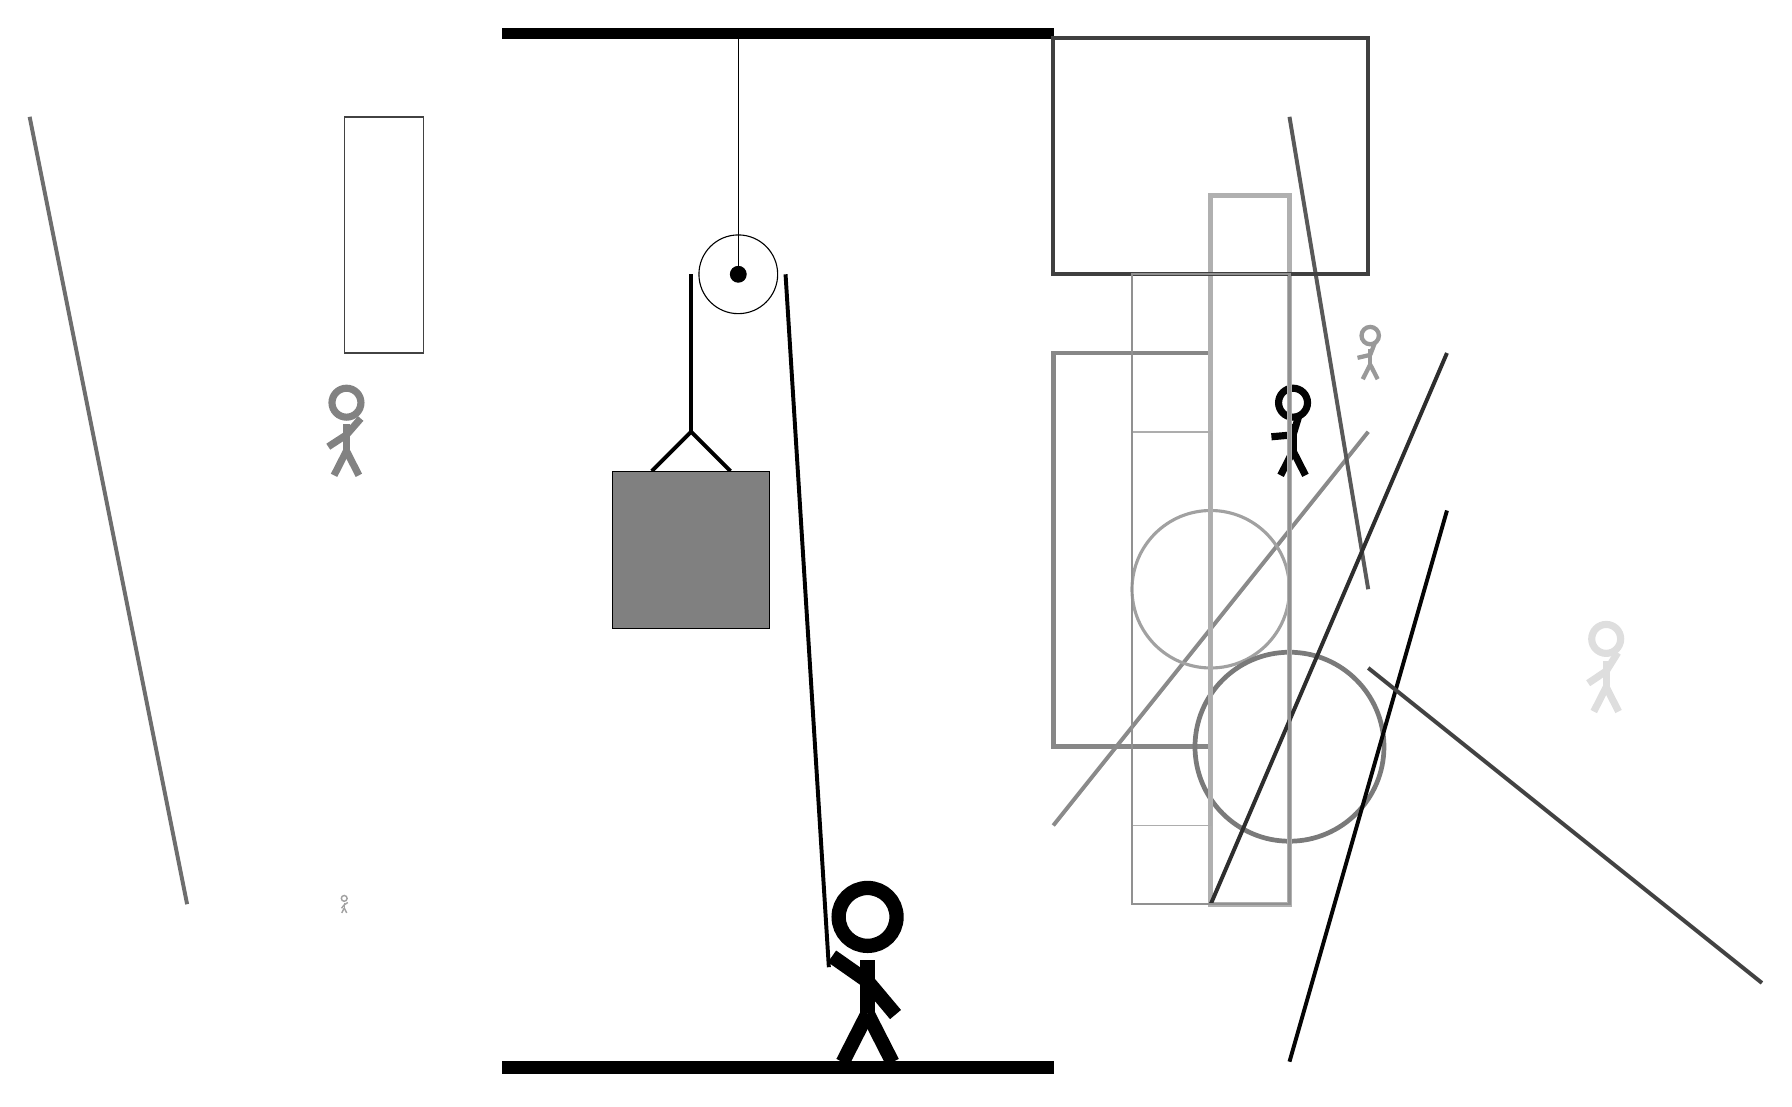
\begin{tikzpicture}
		%%%%% START %%%%%
		
		\draw[fill=black] (-2, 10) rectangle (5, 10.125);
		
		\draw (1, 7) circle (0.5);
		\draw[fill=black] (1, 7) circle (0.1);
		\draw (1, 10) -- (1, 7);
		
		\draw[line width=0.5mm] (-0.1, 4.5) -- (0.4, 5.0) -- (0.9, 4.5);
		\draw[fill=black!50] (-0.6, 4.5) rectangle (1.4, 2.5);
		
		\draw[line width=0.5mm] (0.4, 7) -- (0.4, 5.0);
		\centerarc[line width=0.5mm](1, 7)(0:180:0.6);
		\draw[line width=0.5mm](1.6, 7) -- (2.15, -1.8);
		
		\draw[line width=0.2mm, color=black!74] (-4, 9) rectangle (-3, 6);
		
		\draw[line width=0.6mm, color=black!47] (7, 6) rectangle (5, 1);
		\node[line width=0.4mm, color=black!37] at (-4, -1) {\Strichmaxerl[1][52][33]};
		\draw [line width=0.7mm, color=black!28](12, 3) circle (0.0);
		\draw[line width=0.5mm, color=black!46](9, 5) -- (5, 0);
		
		\draw[line width=0.5mm, color=black!57](-6, -1) -- (-8, 9);
		
		\node[line width=0.3mm, color=black!49] at (-4, 5) {\Strichmaxerl[5][33][49]};
		\node[line width=0.6mm, color=black!40] at (9, 6) {\Strichmaxerl[3][13][69]};
		\node[line width=0.7mm, color=black!99] at (8, 5) {\Strichmaxerl[5][5][73]};
		\draw [line width=0.4mm, color=black!37](7, 3) circle (1.0);
		\draw[line width=0.5mm, color=black!65](8, 9) -- (9, 3);
		\draw [line width=0.6mm, color=black!52](8, 1) circle (1.2);
		\draw[line width=0.6mm, color=black!31] (7, 8) rectangle (8, -1);
		
		\draw[line width=0.5mm, color=black!98](10, 4) -- (8, -3);
		\draw[line width=0.5mm, color=black!82](10, 6) -- (7, -1);
		\draw[line width=0.5mm, color=black!75] (5, 10) rectangle (9, 7);
		
		\draw[line width=0.5mm, color=black!74](9, 2) -- (14, -2);
		
		\draw[line width=0.2mm, color=black!32] (7, 5) rectangle (6, 0);
		\node[line width=0.4mm, color=black!13] at (12, 2) {\Strichmaxerl[5][34][58]};
		
		\draw[line width=0.3mm, color=black!43] (6, 7) rectangle (8, -1);
		
		\node at (2.6, -1.9) {\Strichmaxerl[10][-35][-50]};
		
		\draw[fill=black] (-2, -3) rectangle (5, -3.15);
		
		%%%%% END %%%%%
	\end{tikzpicture}
\end{document}